\section{Algoritmo de Morris-Pratt}

\begin{frame}[fragile]{Motivação}

    \begin{itemize}
        \item No algoritmo de contagem de ocorrências de uma substring $P$ em uma string $S$ por
        busca completa, as comparações feitas entre as substrings $S[i..j]$ e o padrão $P$ 
        são independentes

        \item Isto resulta em várias comparações sendo feitas mais de uma vez e desnecessariamente

        \item Por exemplo, se $S$ = \code{cpp}{"xyzabcdfgh"} e $P$ = \code{cpp}{"abcde"}, a 
            comparação entre a $S[4..8]$ = \code{cpp}{"abcdf"} e o $P$ falha apenas no último 
            caractere (\code{cpp}{'f'} != \code{cpp}{'e'}), localizado no índice 8

        \item Como todos os caracteres de $P$ são distintos, $P$ não pode ocorrer em $S$ a partir 
            dos índices de 5 a 7, mas a busca completa ainda assim realiza tais comparações

        \item O algoritmo de Morris-Pratt explora justamente as comparações entre caracteres já 
            feitas, movendo o índice de ínicio das comparações entre as substrings e o padrão para 
            a posição mais distante possível

    \end{itemize}

\end{frame}

\begin{frame}[fragile]{Conceitos preliminares}

    \begin{itemize}
        \item Um salto seguro $s$ é um inteiro positivo tal que há garantias de que o padrão $P$
            não pode ocorrer entre as posições $i$ e $i + s$ de $S$, mas que pode iniciar-se 
            da posição $i+s$ em diante

        \item Quando o padrão $P$ contém apenas caracteres distintos, é seguro saltar para a 
            posição onde aconteceu a falha

        \item Contudo, é preciso ter cuidado quando há repetições de caracteres no padrão

        \item Mais precisamente, para que o salto seja seguro, deve-se identificar a maior borda 
            possível para $P[1..j]$, de modo a aproveita as comparações bem sucedidas já
            realizadas

        \item O salto deve ser feito para a posição onde esta borda se inicia

    \end{itemize}

\end{frame}

\begin{frame}[fragile]{Conceitos preliminares}

    \begin{itemize}
        \item Considere que $S[i..(i + j - 1)] = P[1..j]$ e que $S[i + j] \neq P[j + 1]$

        \item Assim, o salto seguro $shift(P[1..j])$ de Morris-Pratt para o padrão 
        $P[1..j], j = 1, 2, \ldots, m$ é dado por
        \[
            shift(P[1..j]) = j - |border(P[1..j])|
        \]

        \item Lembre-se de que $border(S)$ é a maior substring própria $B$ de $S$ (isto é,
            $B\neq S$), que é, ao mesmo tempo, sufixo e prefixo de $S$

        \item No caso especial de uma string vazia ($S[i..n]$ e $P$ diferem já no primeiro
            caractere), o salto deve assumir o valor mínimo de 1, de 
            modo que $shift(P[1..0]) = 1$

        \item Logo, se a comparação entre $S[i..n]$ e $P$ falhou na posição $j + 1$ do padrão,
            a próxima comparação a ser feita é entre $P$ e $S[(i + s)..n]$, onde
            $s = shift(P[1..j])$
    \end{itemize}

\end{frame}

\begin{frame}[fragile]{Exemplo de bordas e de saltos seguros}

    \begin{center}
    \begin{tabularx}{0.9\textwidth}{cXcc}
        \toprule
        $j$ & $P[1..j]$ & $border(P[1..j])$ & $shift(P, j)$ \\
        \midrule
        0&\textcolor{red!70}{\verb|""|}&-1&1 \\
        1&\textcolor{red!70}{\verb|"a"|}&0&1 \\
        2&\textcolor{red!70}{\verb|"ab"|}&0&2 \\
        3&\textcolor{red!70}{\verb|"aba"|}&1&2 \\
        4&\textcolor{red!70}{\verb|"abab"|}&2&2 \\
        5&\textcolor{red!70}{\verb|"ababb"|}&0&5 \\
        6&\textcolor{red!70}{\verb|"ababba"|}&1&5 \\
        7&\textcolor{red!70}{\verb|"ababbab"|}&2&5 \\
        8&\textcolor{red!70}{\verb|"ababbaba"|}&3&5 \\
        9&\textcolor{red!70}{\verb|"ababbabab"|}&4&5 \\
        10&\textcolor{red!70}{\verb|"ababbababa"|}&3&7 \\
        11&\textcolor{red!70}{\verb|"ababbababab"|}&4&7 \\
        \bottomrule
    \end{tabularx}
    \end{center}

\end{frame}

\begin{frame}[fragile]{Pseudocódigo do algoritmo de Morris-Pratt}

    \begin{algorithm}[H]
        \caption{Algoritmo de Morris-Pratt}
        \begin{algorithmic}[1]
            \Require Duas strings $P$ e $S$
            \Ensure O número de ocorrências $occ$ de $P$ em $S$

            \Function{Morris-Pratt}{$P$,$S$}
                \State $m \gets |P|, n \gets |S|, occ \gets 0, i \gets 1, j \gets 0$
                \State $bs \gets \Call{borders}{P}$

                \While {$|S[i..n]| \leq m$}
                    \While {$j < m$\algand $P[j + 1] = S[i + j]$}
                        \State $j \gets j + 1$
                    \EndWhile

                    \If {$j = m$}
                        \State $occ \gets occ + 1$
                    \EndIf

                    \State $s \gets j - bs[j]$
                    \State $i \gets i + s$
                    \State $j \gets \max\lbrace 0, bs[j]\rbrace$
                \EndWhile

                \State \Return $occ$
            \EndFunction
        \end{algorithmic}
    \end{algorithm}

\end{frame}

\begin{frame}[fragile]{Visualização do algoritmo de Morris-Pratt}

    \begin{figure}
        \centering

        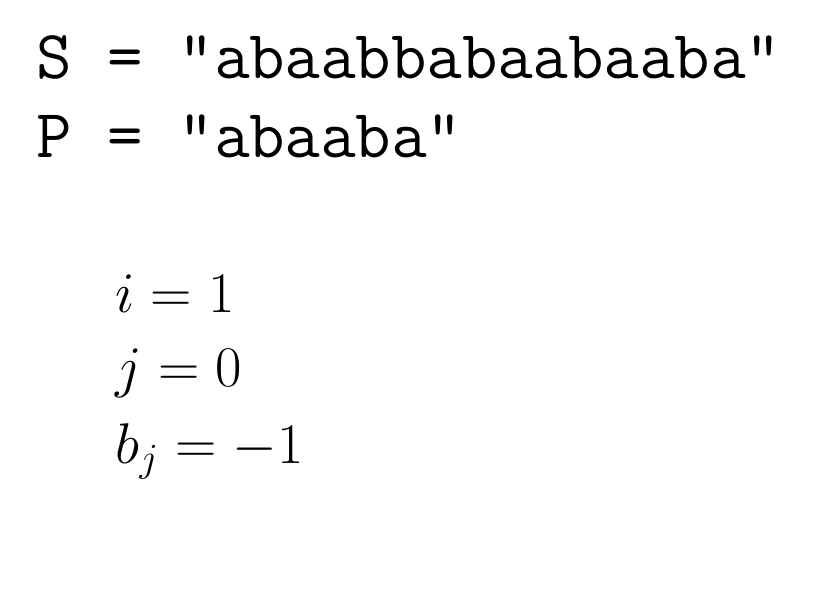
\begin{tikzpicture}
            \node[anchor=west] at (6, 5) { \Huge \texttt{S = "\textcolor{blue}{}abaabbabaabaaba"} };
            \node[anchor=west] at (6, 4) { \Huge \texttt{P = "\textcolor{blue}{}abaaba"} };

            \node[anchor=west] at (7, 2) { \huge $i = 1$ };
            \node[anchor=west] at (7, 1) { \huge $j = 0$ };
            \node[anchor=west] at (7, 0) { \huge $b_j = -1$ };
            \node[opacity=0,anchor=west] at (7, -1) { \huge $s = -1$ };
        \end{tikzpicture}

    \end{figure}

\end{frame}

\begin{frame}[fragile]{Visualização do algoritmo de Morris-Pratt}

    \begin{figure}
        \centering

        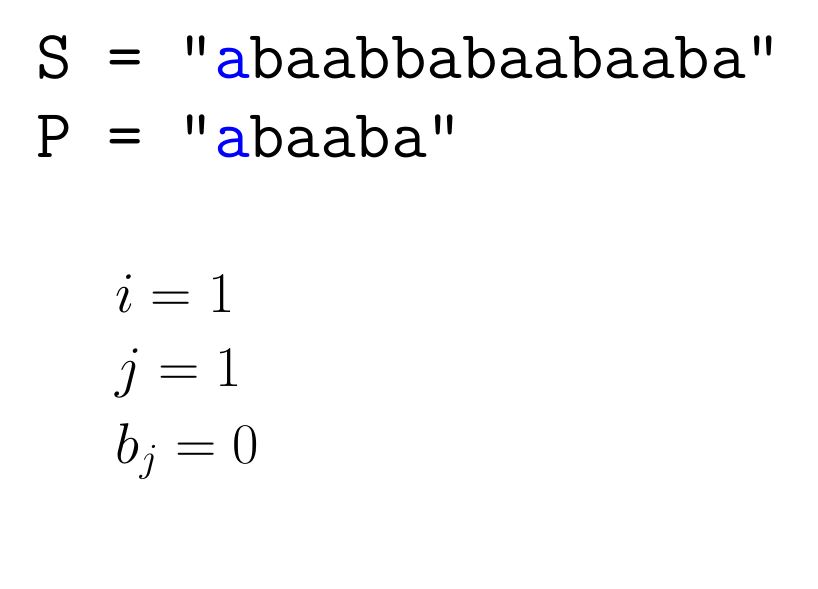
\begin{tikzpicture}
            \node[anchor=west] at (6, 5) { \Huge \texttt{S = "\textcolor{blue}{a}baabbabaabaaba"} };
            \node[anchor=west] at (6, 4) { \Huge \texttt{P = "\textcolor{blue}{a}baaba"} };

            \node[anchor=west] at (7, 2) { \huge $i = 1$ };
            \node[anchor=west] at (7, 1) { \huge $j = 1$ };
            \node[anchor=west] at (7, 0) { \huge $b_j = 0$ };
            \node[opacity=0,anchor=west] at (7, -1) { \huge $s = -1$ };
        \end{tikzpicture}

    \end{figure}

\end{frame}

\begin{frame}[fragile]{Visualização do algoritmo de Morris-Pratt}

    \begin{figure}
        \centering

        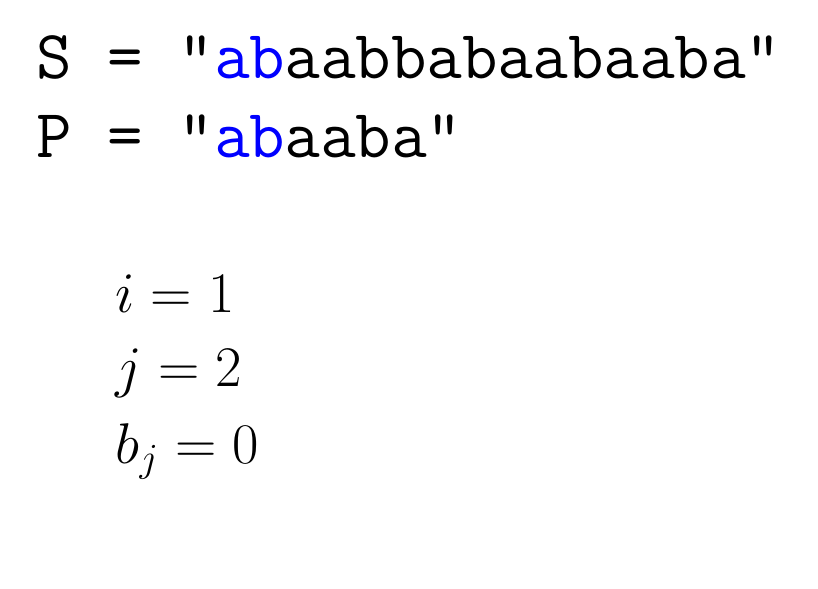
\begin{tikzpicture}
            \node[anchor=west] at (6, 5) { \Huge \texttt{S = "\textcolor{blue}{ab}aabbabaabaaba"} };
            \node[anchor=west] at (6, 4) { \Huge \texttt{P = "\textcolor{blue}{ab}aaba"} };

            \node[anchor=west] at (7, 2) { \huge $i = 1$ };
            \node[anchor=west] at (7, 1) { \huge $j = 2$ };
            \node[anchor=west] at (7, 0) { \huge $b_j = 0$ };
            \node[opacity=0,anchor=west] at (7, -1) { \huge $s = -1$ };
        \end{tikzpicture}

    \end{figure}

\end{frame}

\begin{frame}[fragile]{Visualização do algoritmo de Morris-Pratt}

    \begin{figure}
        \centering

        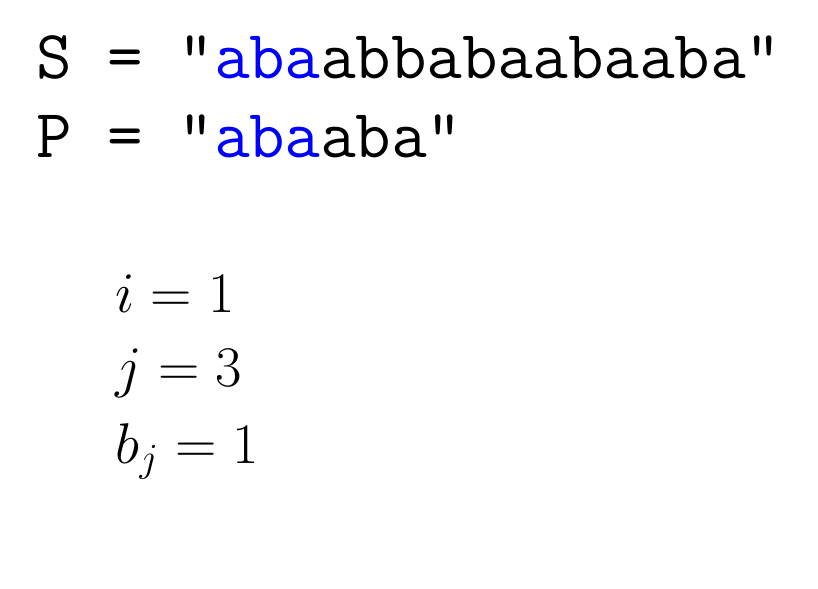
\begin{tikzpicture}
            \node[anchor=west] at (6, 5) { \Huge \texttt{S = "\textcolor{blue}{aba}abbabaabaaba"} };
            \node[anchor=west] at (6, 4) { \Huge \texttt{P = "\textcolor{blue}{aba}aba"} };

            \node[anchor=west] at (7, 2) { \huge $i = 1$ };
            \node[anchor=west] at (7, 1) { \huge $j = 3$ };
            \node[anchor=west] at (7, 0) { \huge $b_j = 1$ };
            \node[opacity=0,anchor=west] at (7, -1) { \huge $s = -1$ };
        \end{tikzpicture}

    \end{figure}

\end{frame}

\begin{frame}[fragile]{Visualização do algoritmo de Morris-Pratt}

    \begin{figure}
        \centering

        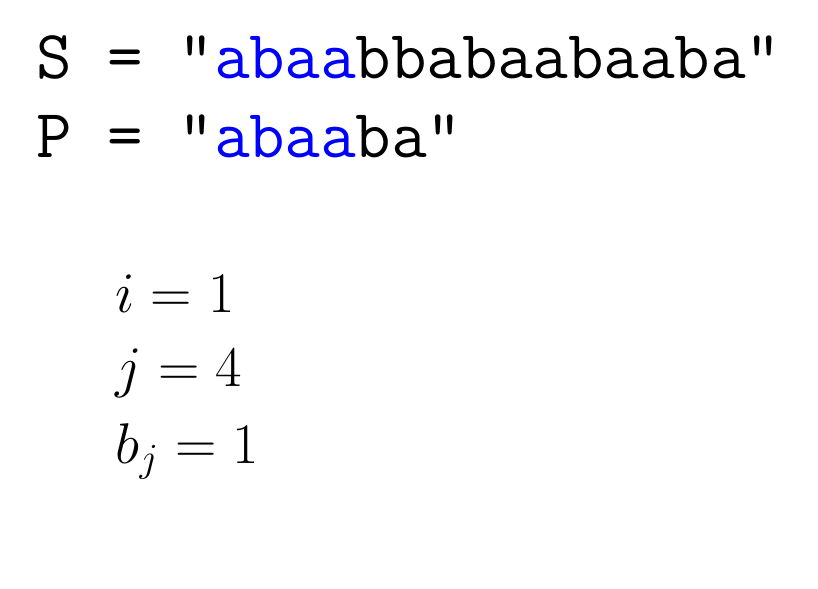
\begin{tikzpicture}
            \node[anchor=west] at (6, 5) { \Huge \texttt{S = "\textcolor{blue}{abaa}bbabaabaaba"} };
            \node[anchor=west] at (6, 4) { \Huge \texttt{P = "\textcolor{blue}{abaa}ba"} };

            \node[anchor=west] at (7, 2) { \huge $i = 1$ };
            \node[anchor=west] at (7, 1) { \huge $j = 4$ };
            \node[anchor=west] at (7, 0) { \huge $b_j = 1$ };
            \node[opacity=0,anchor=west] at (7, -1) { \huge $s = -1$ };
        \end{tikzpicture}

    \end{figure}

\end{frame}

\begin{frame}[fragile]{Visualização do algoritmo de Morris-Pratt}

    \begin{figure}
        \centering

        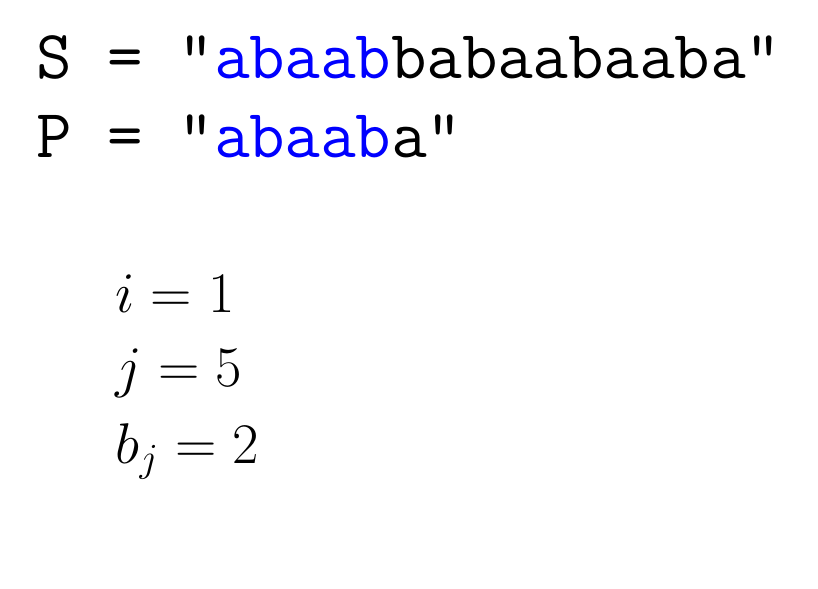
\begin{tikzpicture}
            \node[anchor=west] at (6, 5) { \Huge \texttt{S = "\textcolor{blue}{abaab}babaabaaba"} };
            \node[anchor=west] at (6, 4) { \Huge \texttt{P = "\textcolor{blue}{abaab}a"} };

            \node[anchor=west] at (7, 2) { \huge $i = 1$ };
            \node[anchor=west] at (7, 1) { \huge $j = 5$ };
            \node[anchor=west] at (7, 0) { \huge $b_j = 2$ };
            \node[opacity=0,anchor=west] at (7, -1) { \huge $s = -1$ };
        \end{tikzpicture}

    \end{figure}

\end{frame}

\begin{frame}[fragile]{Visualização do algoritmo de Morris-Pratt}

    \begin{figure}
        \centering

        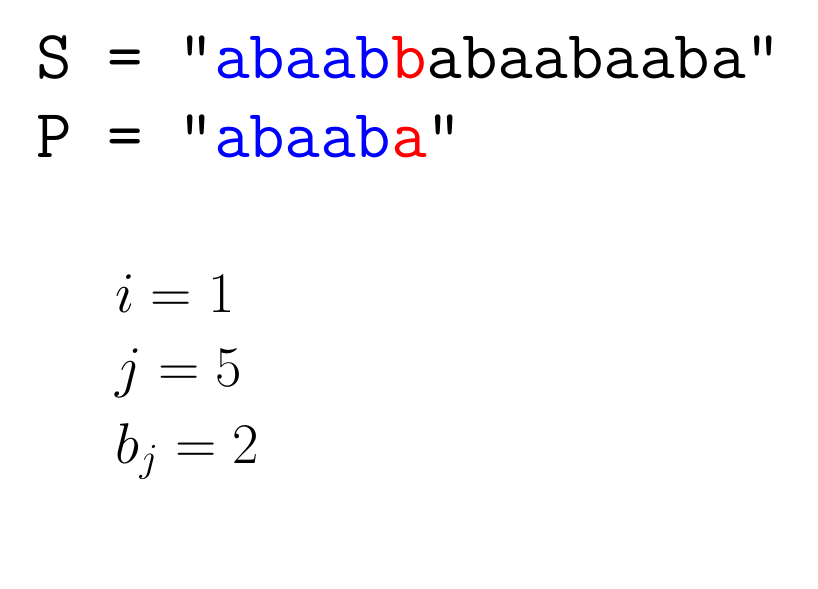
\begin{tikzpicture}
            \node[anchor=west] at (6, 5) { \Huge \texttt{S = "\textcolor{blue}{abaab}\textcolor{red}{b}abaabaaba"} };
            \node[anchor=west] at (6, 4) { \Huge \texttt{P = "\textcolor{blue}{abaab}\textcolor{red}{a}"} };

            \node[anchor=west] at (7, 2) { \huge $i = 1$ };
            \node[anchor=west] at (7, 1) { \huge $j = 5$ };
            \node[anchor=west] at (7, 0) { \huge $b_j = 2$ };
            \node[opacity=0,anchor=west] at (7, -1) { \huge $s = -1$ };
        \end{tikzpicture}

    \end{figure}

\end{frame}

\begin{frame}[fragile]{Visualização do algoritmo de Morris-Pratt}

    \begin{figure}
        \centering

        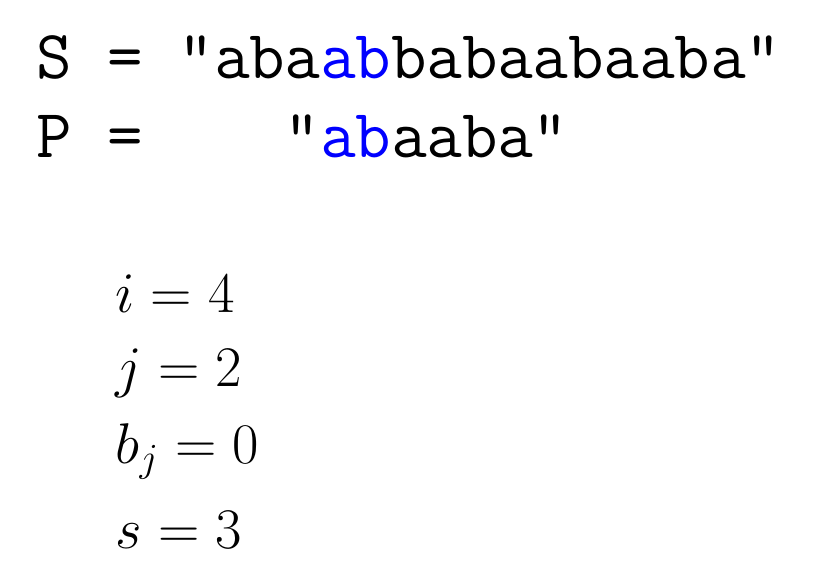
\begin{tikzpicture}
            \node[anchor=west] at (6, 5) { \Huge \texttt{S = "aba\textcolor{blue}{ab}\textcolor{red}{}babaabaaba"} };
            \node[anchor=west] at (6, 4) { \Huge \texttt{P = \ \ \ "\textcolor{blue}{ab}aaba"} };

            \node[anchor=west] at (7, 2) { \huge $i = 4$ };
            \node[anchor=west] at (7, 1) { \huge $j = 2$ };
            \node[anchor=west] at (7, 0) { \huge $b_j = 0$ };
            \node[opacity=1,anchor=west] at (7, -1) { \huge $s = 3$ };
        \end{tikzpicture}

    \end{figure}

\end{frame}

\begin{frame}[fragile]{Visualização do algoritmo de Morris-Pratt}

    \begin{figure}
        \centering

        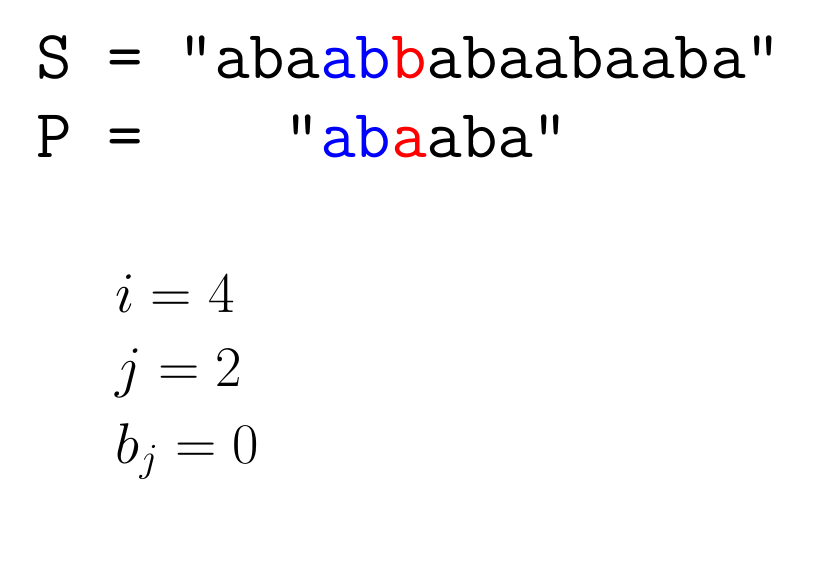
\begin{tikzpicture}
            \node[anchor=west] at (6, 5) { \Huge \texttt{S = "aba\textcolor{blue}{ab}\textcolor{red}{b}abaabaaba"} };
            \node[anchor=west] at (6, 4) { \Huge \texttt{P = \ \ \ "\textcolor{blue}{ab}\textcolor{red}{a}aba"} };

            \node[anchor=west] at (7, 2) { \huge $i = 4$ };
            \node[anchor=west] at (7, 1) { \huge $j = 2$ };
            \node[anchor=west] at (7, 0) { \huge $b_j = 0$ };
            \node[opacity=0,anchor=west] at (7, -1) { \huge $s = 3$ };
        \end{tikzpicture}

    \end{figure}

\end{frame}

\begin{frame}[fragile]{Visualização do algoritmo de Morris-Pratt}

    \begin{figure}
        \centering

        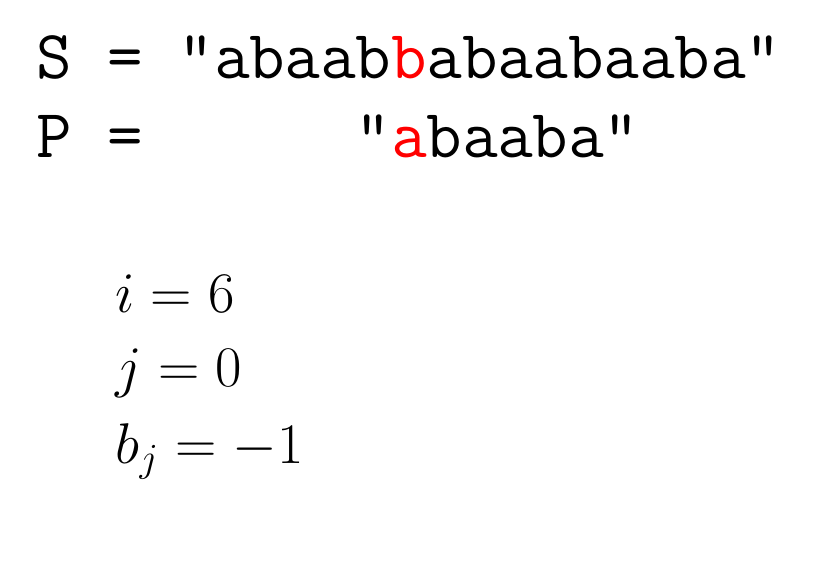
\begin{tikzpicture}
            \node[anchor=west] at (6, 5) { \Huge \texttt{S = "abaab\textcolor{blue}{}\textcolor{red}{b}abaabaaba"} };
            \node[anchor=west] at (6, 4) { \Huge \texttt{P = \ \ \ \ \ "\textcolor{blue}{}\textcolor{red}{a}baaba"} };

            \node[anchor=west] at (7, 2) { \huge $i = 6$ };
            \node[anchor=west] at (7, 1) { \huge $j = 0$ };
            \node[anchor=west] at (7, 0) { \huge $b_j = -1$ };
            \node[opacity=0,anchor=west] at (7, -1) { \huge $s = 2$ };
        \end{tikzpicture}

    \end{figure}

\end{frame}

\begin{frame}[fragile]{Visualização do algoritmo de Morris-Pratt}

    \begin{figure}
        \centering

        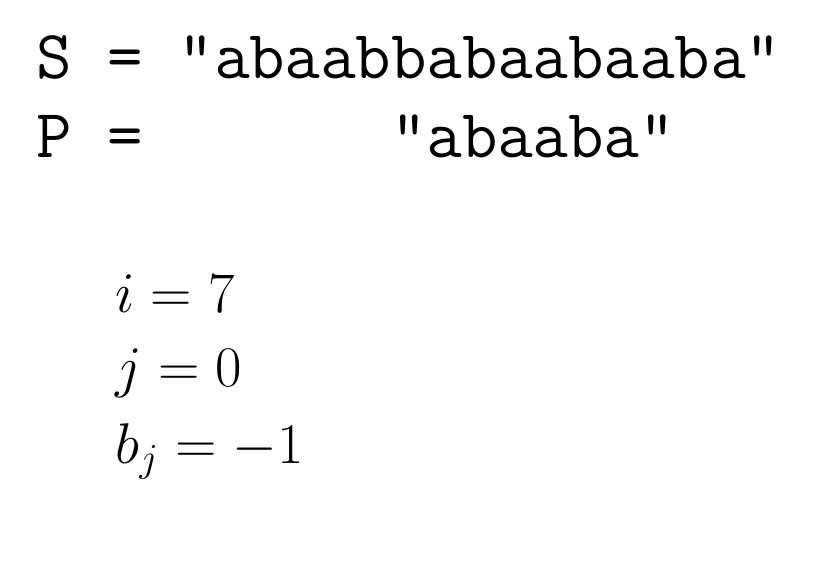
\begin{tikzpicture}
            \node[anchor=west] at (6, 5) { \Huge \texttt{S = "abaabb\textcolor{blue}{}\textcolor{red}{}abaabaaba"} };
            \node[anchor=west] at (6, 4) { \Huge \texttt{P = \ \ \ \ \ \ "\textcolor{blue}{}\textcolor{red}{}abaaba"} };

            \node[anchor=west] at (7, 2) { \huge $i = 7$ };
            \node[anchor=west] at (7, 1) { \huge $j = 0$ };
            \node[anchor=west] at (7, 0) { \huge $b_j = -1$ };
            \node[opacity=0,anchor=west] at (7, -1) { \huge $s = 1$ };
        \end{tikzpicture}

    \end{figure}

\end{frame}

\begin{frame}[fragile]{Visualização do algoritmo de Morris-Pratt}

    \begin{figure}
        \centering

        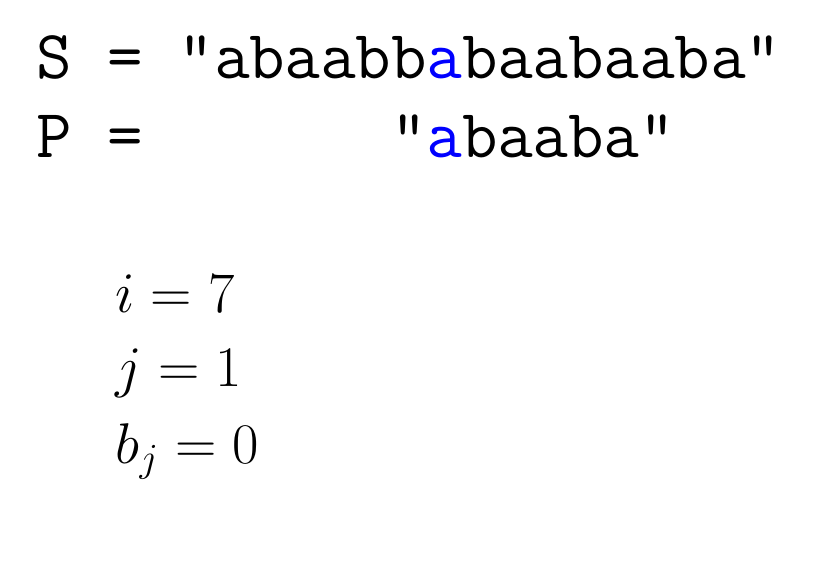
\begin{tikzpicture}
            \node[anchor=west] at (6, 5) { \Huge \texttt{S = "abaabb\textcolor{blue}{a}\textcolor{red}{}baabaaba"} };
            \node[anchor=west] at (6, 4) { \Huge \texttt{P = \ \ \ \ \ \ "\textcolor{blue}{a}\textcolor{red}{}baaba"} };

            \node[anchor=west] at (7, 2) { \huge $i = 7$ };
            \node[anchor=west] at (7, 1) { \huge $j = 1$ };
            \node[anchor=west] at (7, 0) { \huge $b_j = 0$ };
            \node[opacity=0,anchor=west] at (7, -1) { \huge $s = 1$ };
        \end{tikzpicture}

    \end{figure}

\end{frame}

\begin{frame}[fragile]{Visualização do algoritmo de Morris-Pratt}

    \begin{figure}
        \centering

        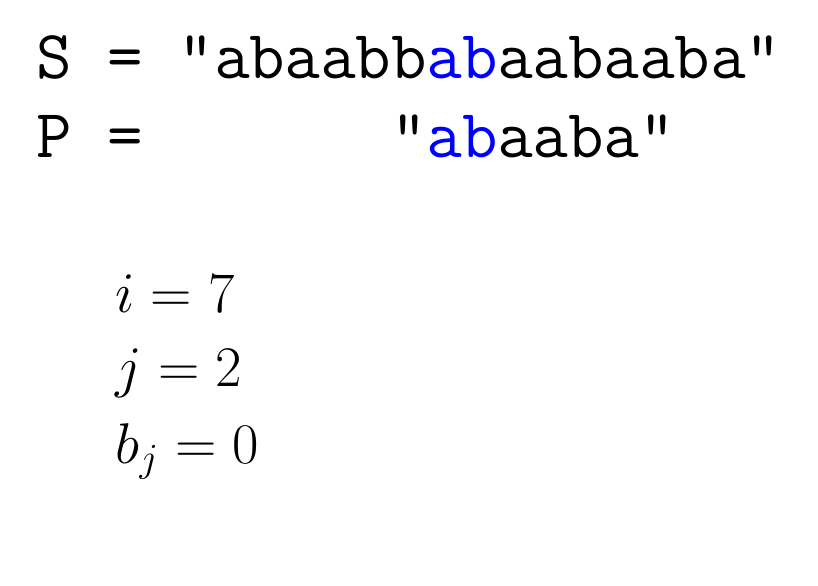
\begin{tikzpicture}
            \node[anchor=west] at (6, 5) { \Huge \texttt{S = "abaabb\textcolor{blue}{ab}\textcolor{red}{}aabaaba"} };
            \node[anchor=west] at (6, 4) { \Huge \texttt{P = \ \ \ \ \ \ "\textcolor{blue}{ab}\textcolor{red}{}aaba"} };

            \node[anchor=west] at (7, 2) { \huge $i = 7$ };
            \node[anchor=west] at (7, 1) { \huge $j = 2$ };
            \node[anchor=west] at (7, 0) { \huge $b_j = 0$ };
            \node[opacity=0,anchor=west] at (7, -1) { \huge $s = 1$ };
        \end{tikzpicture}

    \end{figure}

\end{frame}

\begin{frame}[fragile]{Visualização do algoritmo de Morris-Pratt}

    \begin{figure}
        \centering

        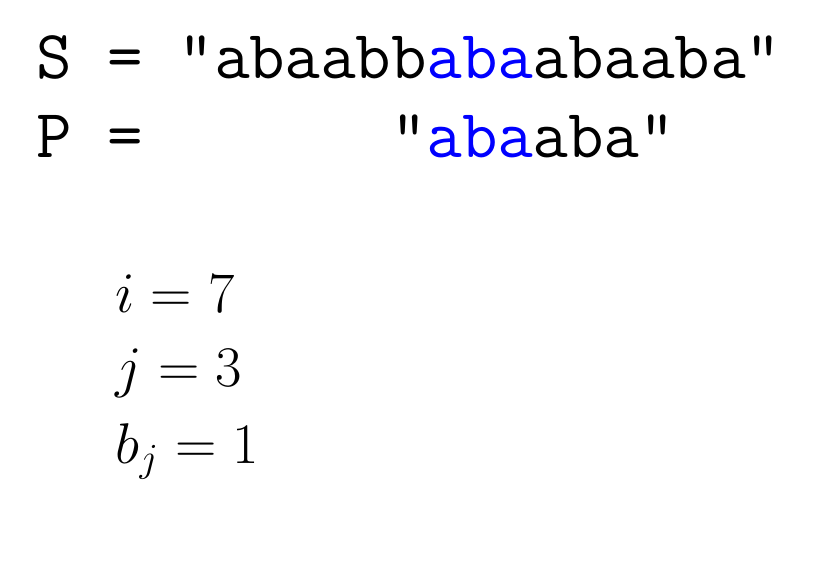
\begin{tikzpicture}
            \node[anchor=west] at (6, 5) { \Huge \texttt{S = "abaabb\textcolor{blue}{aba}\textcolor{red}{}abaaba"} };
            \node[anchor=west] at (6, 4) { \Huge \texttt{P = \ \ \ \ \ \ "\textcolor{blue}{aba}\textcolor{red}{}aba"} };

            \node[anchor=west] at (7, 2) { \huge $i = 7$ };
            \node[anchor=west] at (7, 1) { \huge $j = 3$ };
            \node[anchor=west] at (7, 0) { \huge $b_j = 1$ };
            \node[opacity=0,anchor=west] at (7, -1) { \huge $s = 1$ };
        \end{tikzpicture}

    \end{figure}

\end{frame}

\begin{frame}[fragile]{Visualização do algoritmo de Morris-Pratt}

    \begin{figure}
        \centering

        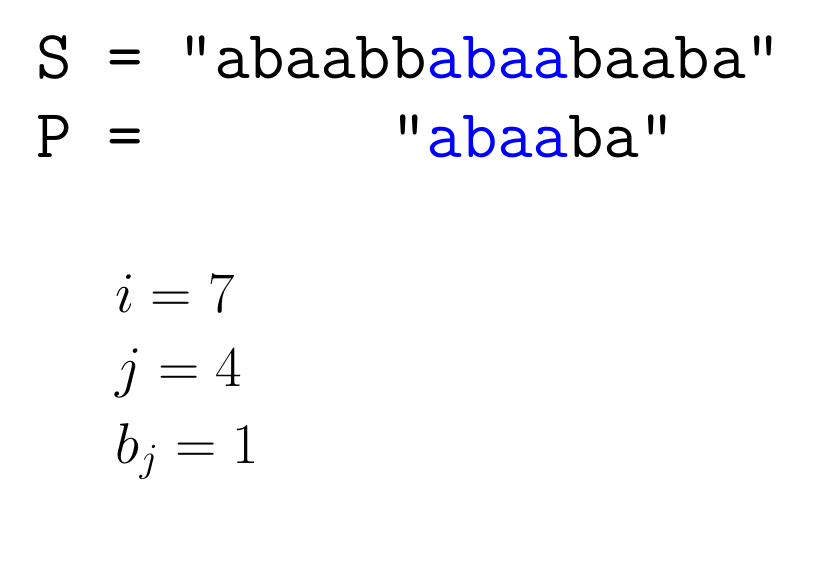
\begin{tikzpicture}
            \node[anchor=west] at (6, 5) { \Huge \texttt{S = "abaabb\textcolor{blue}{abaa}\textcolor{red}{}baaba"} };
            \node[anchor=west] at (6, 4) { \Huge \texttt{P = \ \ \ \ \ \ "\textcolor{blue}{abaa}\textcolor{red}{}ba"} };

            \node[anchor=west] at (7, 2) { \huge $i = 7$ };
            \node[anchor=west] at (7, 1) { \huge $j = 4$ };
            \node[anchor=west] at (7, 0) { \huge $b_j = 1$ };
            \node[opacity=0,anchor=west] at (7, -1) { \huge $s = 1$ };
        \end{tikzpicture}

    \end{figure}

\end{frame}

\begin{frame}[fragile]{Visualização do algoritmo de Morris-Pratt}

    \begin{figure}
        \centering

        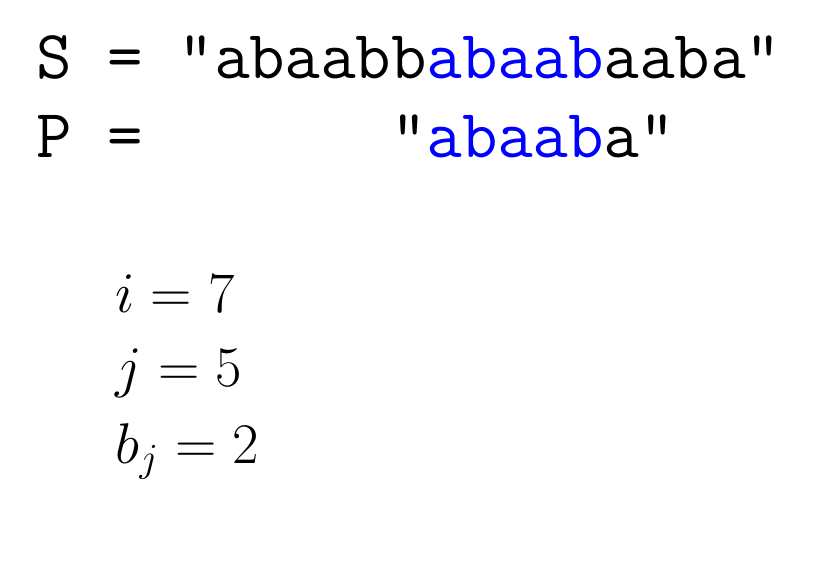
\begin{tikzpicture}
            \node[anchor=west] at (6, 5) { \Huge \texttt{S = "abaabb\textcolor{blue}{abaab}\textcolor{red}{}aaba"} };
            \node[anchor=west] at (6, 4) { \Huge \texttt{P = \ \ \ \ \ \ "\textcolor{blue}{abaab}\textcolor{red}{}a"} };

            \node[anchor=west] at (7, 2) { \huge $i = 7$ };
            \node[anchor=west] at (7, 1) { \huge $j = 5$ };
            \node[anchor=west] at (7, 0) { \huge $b_j = 2$ };
            \node[opacity=0,anchor=west] at (7, -1) { \huge $s = 1$ };
        \end{tikzpicture}

    \end{figure}

\end{frame}

\begin{frame}[fragile]{Visualização do algoritmo de Morris-Pratt}

    \begin{figure}
        \centering

        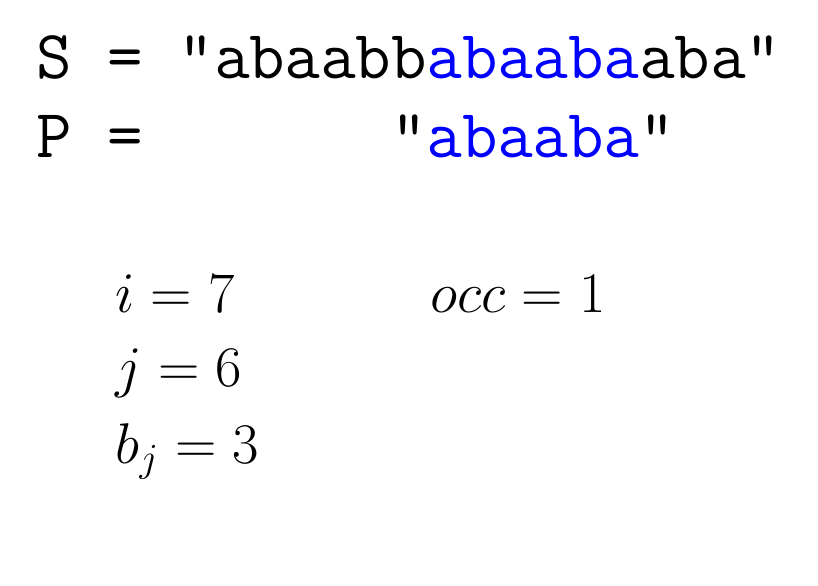
\begin{tikzpicture}
            \node[anchor=west] at (6, 5) { \Huge \texttt{S = "abaabb\textcolor{blue}{abaaba}\textcolor{red}{}aba"} };
            \node[anchor=west] at (6, 4) { \Huge \texttt{P = \ \ \ \ \ \ "\textcolor{blue}{abaaba}\textcolor{red}{}"} };

            \node[anchor=west] at (7, 2) { \huge $i = 7$ };
            \node[anchor=west] at (11, 2) { \huge $occ = 1$ };
            \node[anchor=west] at (7, 1) { \huge $j = 6$ };
            \node[anchor=west] at (7, 0) { \huge $b_j = 3$ };
            \node[opacity=0,anchor=west] at (7, -1) { \huge $s = 1$ };
        \end{tikzpicture}

    \end{figure}

\end{frame}

\begin{frame}[fragile]{Visualização do algoritmo de Morris-Pratt}

    \begin{figure}
        \centering

        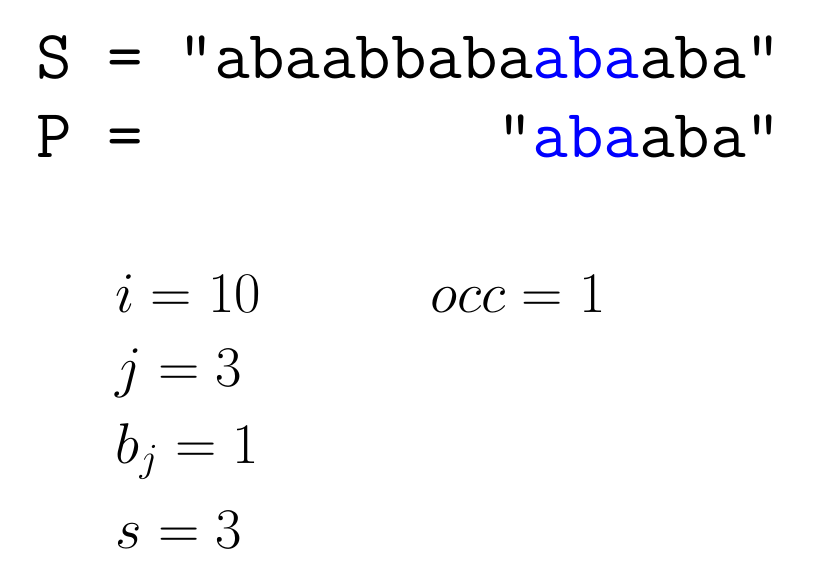
\begin{tikzpicture}
            \node[anchor=west] at (6, 5) { \Huge \texttt{S = "abaabbaba\textcolor{blue}{aba}\textcolor{red}{}aba"} };
            \node[anchor=west] at (6, 4) { \Huge \texttt{P = \ \ \ \ \ \ \ \ \ "\textcolor{blue}{aba}aba"} };

            \node[anchor=west] at (7, 2) { \huge $i = 10$ };
            \node[anchor=west] at (11, 2) { \huge $occ = 1$ };
            \node[anchor=west] at (7, 1) { \huge $j = 3$ };
            \node[anchor=west] at (7, 0) { \huge $b_j = 1$ };
            \node[opacity=1,anchor=west] at (7, -1) { \huge $s = 3$ };
        \end{tikzpicture}

    \end{figure}

\end{frame}

\begin{frame}[fragile]{Visualização do algoritmo de Morris-Pratt}

    \begin{figure}
        \centering

        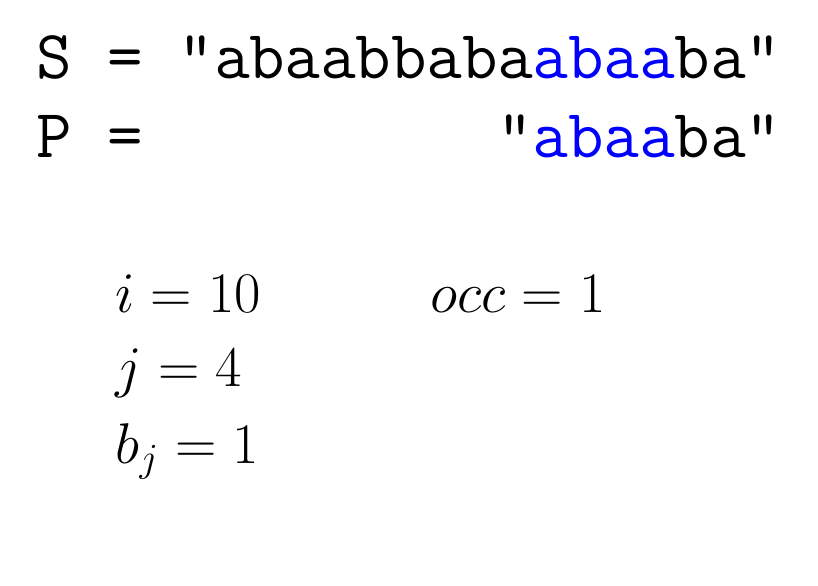
\begin{tikzpicture}
            \node[anchor=west] at (6, 5) { \Huge \texttt{S = "abaabbaba\textcolor{blue}{abaa}\textcolor{red}{}ba"} };
            \node[anchor=west] at (6, 4) { \Huge \texttt{P = \ \ \ \ \ \ \ \ \ "\textcolor{blue}{abaa}ba"} };

            \node[anchor=west] at (7, 2) { \huge $i = 10$ };
            \node[anchor=west] at (11, 2) { \huge $occ = 1$ };
            \node[anchor=west] at (7, 1) { \huge $j = 4$ };
            \node[anchor=west] at (7, 0) { \huge $b_j = 1$ };
            \node[opacity=0,anchor=west] at (7, -1) { \huge $s = 3$ };
        \end{tikzpicture}

    \end{figure}

\end{frame}

\begin{frame}[fragile]{Visualização do algoritmo de Morris-Pratt}

    \begin{figure}
        \centering

        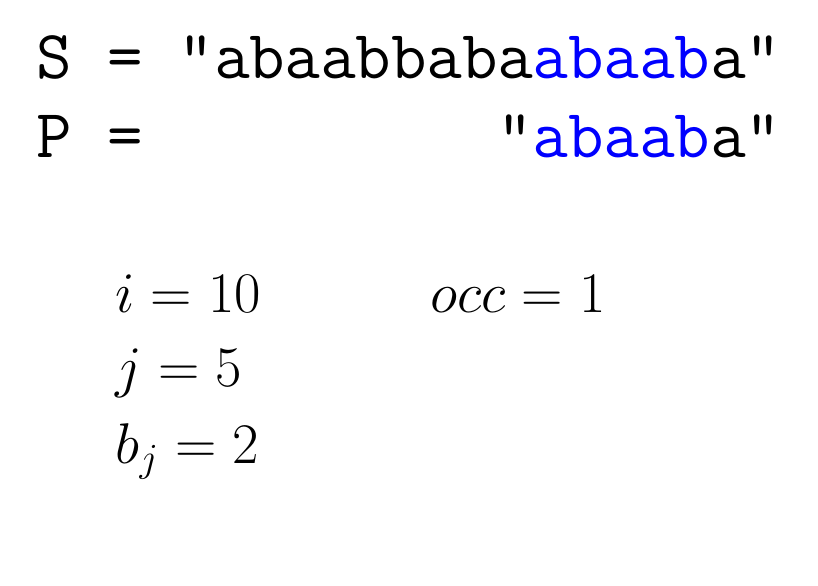
\begin{tikzpicture}
            \node[anchor=west] at (6, 5) { \Huge \texttt{S = "abaabbaba\textcolor{blue}{abaab}\textcolor{red}{}a"} };
            \node[anchor=west] at (6, 4) { \Huge \texttt{P = \ \ \ \ \ \ \ \ \ "\textcolor{blue}{abaab}a"} };

            \node[anchor=west] at (7, 2) { \huge $i = 10$ };
            \node[anchor=west] at (11, 2) { \huge $occ = 1$ };
            \node[anchor=west] at (7, 1) { \huge $j = 5$ };
            \node[anchor=west] at (7, 0) { \huge $b_j = 2$ };
            \node[opacity=0,anchor=west] at (7, -1) { \huge $s = 3$ };
        \end{tikzpicture}

    \end{figure}

\end{frame}

\begin{frame}[fragile]{Visualização do algoritmo de Morris-Pratt}

    \begin{figure}
        \centering

        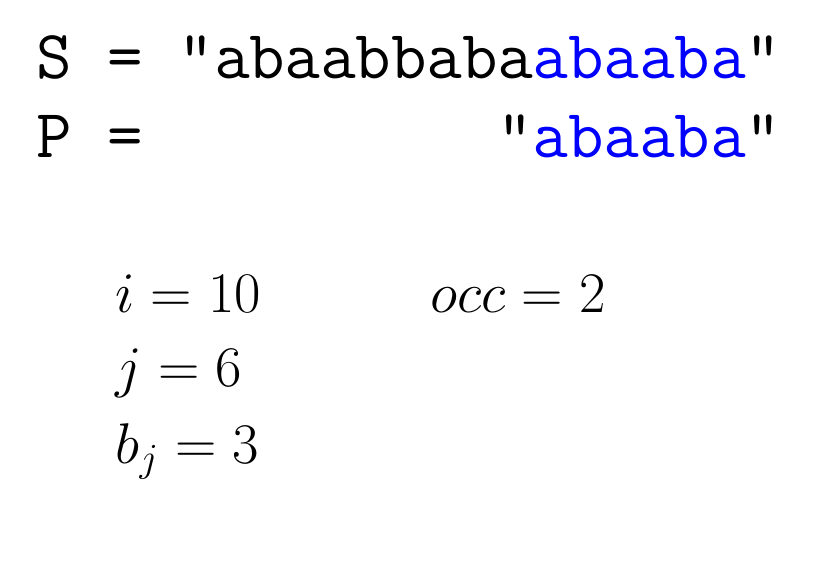
\begin{tikzpicture}
            \node[anchor=west] at (6, 5) { \Huge \texttt{S = "abaabbaba\textcolor{blue}{abaaba}\textcolor{red}{}"} };
            \node[anchor=west] at (6, 4) { \Huge \texttt{P = \ \ \ \ \ \ \ \ \ "\textcolor{blue}{abaaba}"} };

            \node[anchor=west] at (7, 2) { \huge $i = 10$ };
            \node[anchor=west] at (11, 2) { \huge $occ = 2$ };
            \node[anchor=west] at (7, 1) { \huge $j = 6$ };
            \node[anchor=west] at (7, 0) { \huge $b_j = 3$ };
            \node[opacity=0,anchor=west] at (7, -1) { \huge $s = 3$ };
        \end{tikzpicture}

    \end{figure}

\end{frame}


\begin{frame}[fragile]{Complexidade do algoritmo de Morris-Pratt}

    \begin{itemize}
        \item O algoritmo de Morris-Pratt realiza, no máximo, um número de comparações linear em 
            termos dos tamanhos de $S$ e $P$, a saber, $2n - m$ comparações

        \item Isto porque a comparação $P[j + 1] = S[i + j]$ pode falhar, no máximo, 
            $n - m + 1$ vezes, já que o primeiro laço é executado $n - m + 1$ vezes, e pode ter 
            sucesso, no máximo, $n$ vezes, quando o $S$ e $P$ são compostos por um mesmo
            caractere

        \item Caso a primeira comparação seja bem sucedida, ela não pode falhar no índice 0

        \item O pior caso, em termos de número de comparações, acontece quando $P$ é formado
            por  apenas duas letras distinas e $S$ é uma repetição de $n - 1$ vezes a primeira 
            letra de $P$ e a última letra é igual a segunda letra de $P$
    \end{itemize}

\end{frame}

\begin{frame}[fragile]{Complexidade do algoritmo de Morris-Pratt}

    \begin{itemize}
        \item Por exemplo, $P$ = \code{cpp}{"ab"} e $S$ = \code{cpp}{"aaaaaaaaaaaab"}

        \item Neste caso, a primeira comparação será bem sucedida $n - 1$ vezes, haverão $n - 2$
        falhas (em relação ao último caractere do padrão) e uma última comparação bem sucedida no 
        último caractere

        \item Daí o máximo de comparações será igual a 
        \[
            (n - 1) + (n - 2) + 1 = 2n - 2 = 2n - m
        \]

        \item Assim, o algoritmo MP é linear em relação ao tamanho do texto

        \item Porém, para determinar sua complexidade, falta determinar a complexidade da 
            construção do vetor $bs$

        \item Se a construção de $bs$ tem complexidade $O(m)$, o algoritmo de Morris-Pratt tem
            complexidade $O(n + m)$ no pior caso
    \end{itemize}

\end{frame}

\begin{frame}[fragile]{Cálculo das bordas de $S$}

    \begin{itemize}
        \item Observe que
        \[
            border(S), border^2(S), \ldots, border^k(S),
        \]
        com $border^k(S) = $ \code{cpp}{""}, é uma sequência de strings, decrescente em relação
        ao tamanho, cujos elementos são todos bordas de $S$

        \item Este fato permite o cálculo de $b_j = |border(P[1..j])|$ para todos os prefixos de 
            $P$ em $O(m)$

        \item Observe que, $P[j + 1] = P[b_j + 1]$, então 
        \[
            b_{j + 1} = 1 + b_j
        \]

        \item Isto porque a maior borda de $P[1..j]$ tem tamanho $b_j$, então se o caractere
            $P[j + 1]$ coincidir com o caractere que sucede o prefixo que forma a borda, 
            a maior borda de $P[1..(j+1)]$  será uma unidade maior do que a maior borda de $P[1..j]$
    \end{itemize}

\end{frame}

\begin{frame}[fragile]{Cálculo das bordas de $S$}

    \begin{itemize}
        \item Se $P[j + 1] \neq P[b_j + 1]$, então a borda de $P[j + 1]$ deve ser reavaliada
            em termos da segunda maior borda de $P[1..j]$, isto é,
        \[
            b_{j + 1} = 1 + |border^2(P)| = 1 + b_j^2
        \]
        se $P[j + 1] = P[b_j^2 + 1]$

        \item Caso $P[j + 1] \neq P[b_j^2 + 1]$, o raciocínio se repete até atingir a $k$-ésima
            borda de $P$

        \item Portanto,
        \[
            b_{j + 1} = 1 + \max \lbrace\ border^i(P)\ |\ P[j + 1] = P[b_j^i + 1], i\in [1..k]\ \rbrace
        \]

        \item O caso base acontece no prefixo vazio, isto é, $P[1..0] = $ \code{cpp}{""}, onde
            $b_0 = -1$, por conta do termo $+1$ na recorrência anterior

    \end{itemize}

\end{frame}

\begin{frame}[fragile]{Implementação do algoritmo de Morris-Pratt em C++}
    \inputsnippet{cpp}{1}{20}{codes/mp.cpp}
\end{frame}

\begin{frame}[fragile]{Implementação do algoritmo de Morris-Pratt em C++}
    \inputsnippet{cpp}{22}{41}{codes/mp.cpp}
\end{frame}
